\subsection{lema-teo-fundamental-da-algebra} 
\label{lema-teo-fundamental-da-algebra}
\begin{titlemize}{Lista de dependências}
	\item \hyperref[homotopia]{homotopia};\\  
	\item \hyperref[grupo-fundamental]{grupo-fundamental};\\
    \item \hyperref[retração]{retração};

\end{titlemize}
O próximo lema será uma das bases para a demonstração do Teorema Fundamental da Álgebra.
\begin{thm}[Lema] 
	Seja $\mathbb{C}$ o conjunto dos números complexos e $r\mathbb{S}^1 \subseteq \mathbb{R}^2 \cong \mathbb{C}$ a esfera centrada em 0 e de raio $r$. Sejam $f_r^n: r\mathbb{S}^1 \rightarrow \mathbb{C}\backslash \{0\}$ as restrições das funções que levam $z$ em $z^n$. Se nenhuma das funções é homotópica a uma função constante, então vale o Teorema Fundamental da Álgebra, ou seja, todo polinômio com grau maior ou igual a 1 tem raiz complexa.
	
\end{thm}

\begin{dem}
    Seja $g(z) = a_nz^n + a_{n - 1}z^{n - 1} +...+ a_0$
um polinômio com raízes complexas e com $a_n \neq 0$. Sem perda de generalidade, podemos supor $a_n = 1$ (basta tomar $h(z) = \frac{g(z)}{a_n}$).\\ Seja $r > max\{1, \sum_{i = 1}^n|a_i|\}$ e defino $F:r\mathbb{S}^1\times I \rightarrow \mathbb{C}$ como

$$F(z, t) = z^n + \sum_{i = 1}^{n-1}(1 - t)a_iz^i$$

Nota-se facilmente que $F$ é homotopia de $f_r^n$ e $g|_{r\mathbb{S}^1}$. Ainda, o contradomínio da $F$ é $\mathbb{C}\backslash \{0\}$, pois se não, haveria $z_0$ com $|z_0| = r$ e $t_0 \in I$, tal que $F(z_0, t_0) = 0$, i.e. $z_0^n = -\sum_{i = 1}^{n - 1}(1 - t_0)a_iz^i$ e, então, 

$$|z_o^n| = r^n \leq \sum_{i = 1}^{n - 1}|(1 - t_0)a_iz_0^i| \leq \sum_{i = 1}^{n - 1}|a_iz_0^i| \leq r^{n-1}\sum_{i = 1}^{n - 1}|a_i|$$

que implicaria $r \leq \sum_{i = 1}^{n - 1}|a_i|$, contradizendo a escolha de $r$.

Agora, por contrapositiva, assumimos que $g$ não tem raízes complexas, i.e. $g:\mathbb{C} \rightarrow \mathbb{C}\backslash\{0\}$. Seja $G: r\mathbb{S}^1\times I \rightarrow \mathbb{C}\backslash\{0\}$ definida por $g((1 - t)z)$. Temos que $g \sim_G c$, onde $c(z) = g(0) = a_0$ para todo $z \in r\mathbb{S}^1$. Assim, temos que $f_r^n \sim_G c$ por transitividade, garantindo a contrapositiva.  

\end{dem}
A restrição no contradomínio da $f_r^n$ é importante, pois se o contradomínio for contrátil, então qualquer função é homotópica a uma constante. De fato, se $f:X \rightarrow Y$ e $Y$ é contrátil, então $1_Y \sim_H k$, onde $k$ é uma função constante e $H$ é homotopia. Então, $f\circ1_Y \sim_H f\circ k$ e, portanto, $f \sim_H f(k_0)$, onde $k_0 = k(z)$. \\

Note também que a homotopia de $g|_{r\mathbb{S}^1}$ e $f_r^n$ deforma continuamente a imagem do polinômio que, restrito a $r\mathbb{S}^1$, torna-se uma curva fechada no plano dos complexos, no círculo de raio $r$ em $\mathbb{C}$. Veja a imagem abaixo.

\begin{figure}[h]
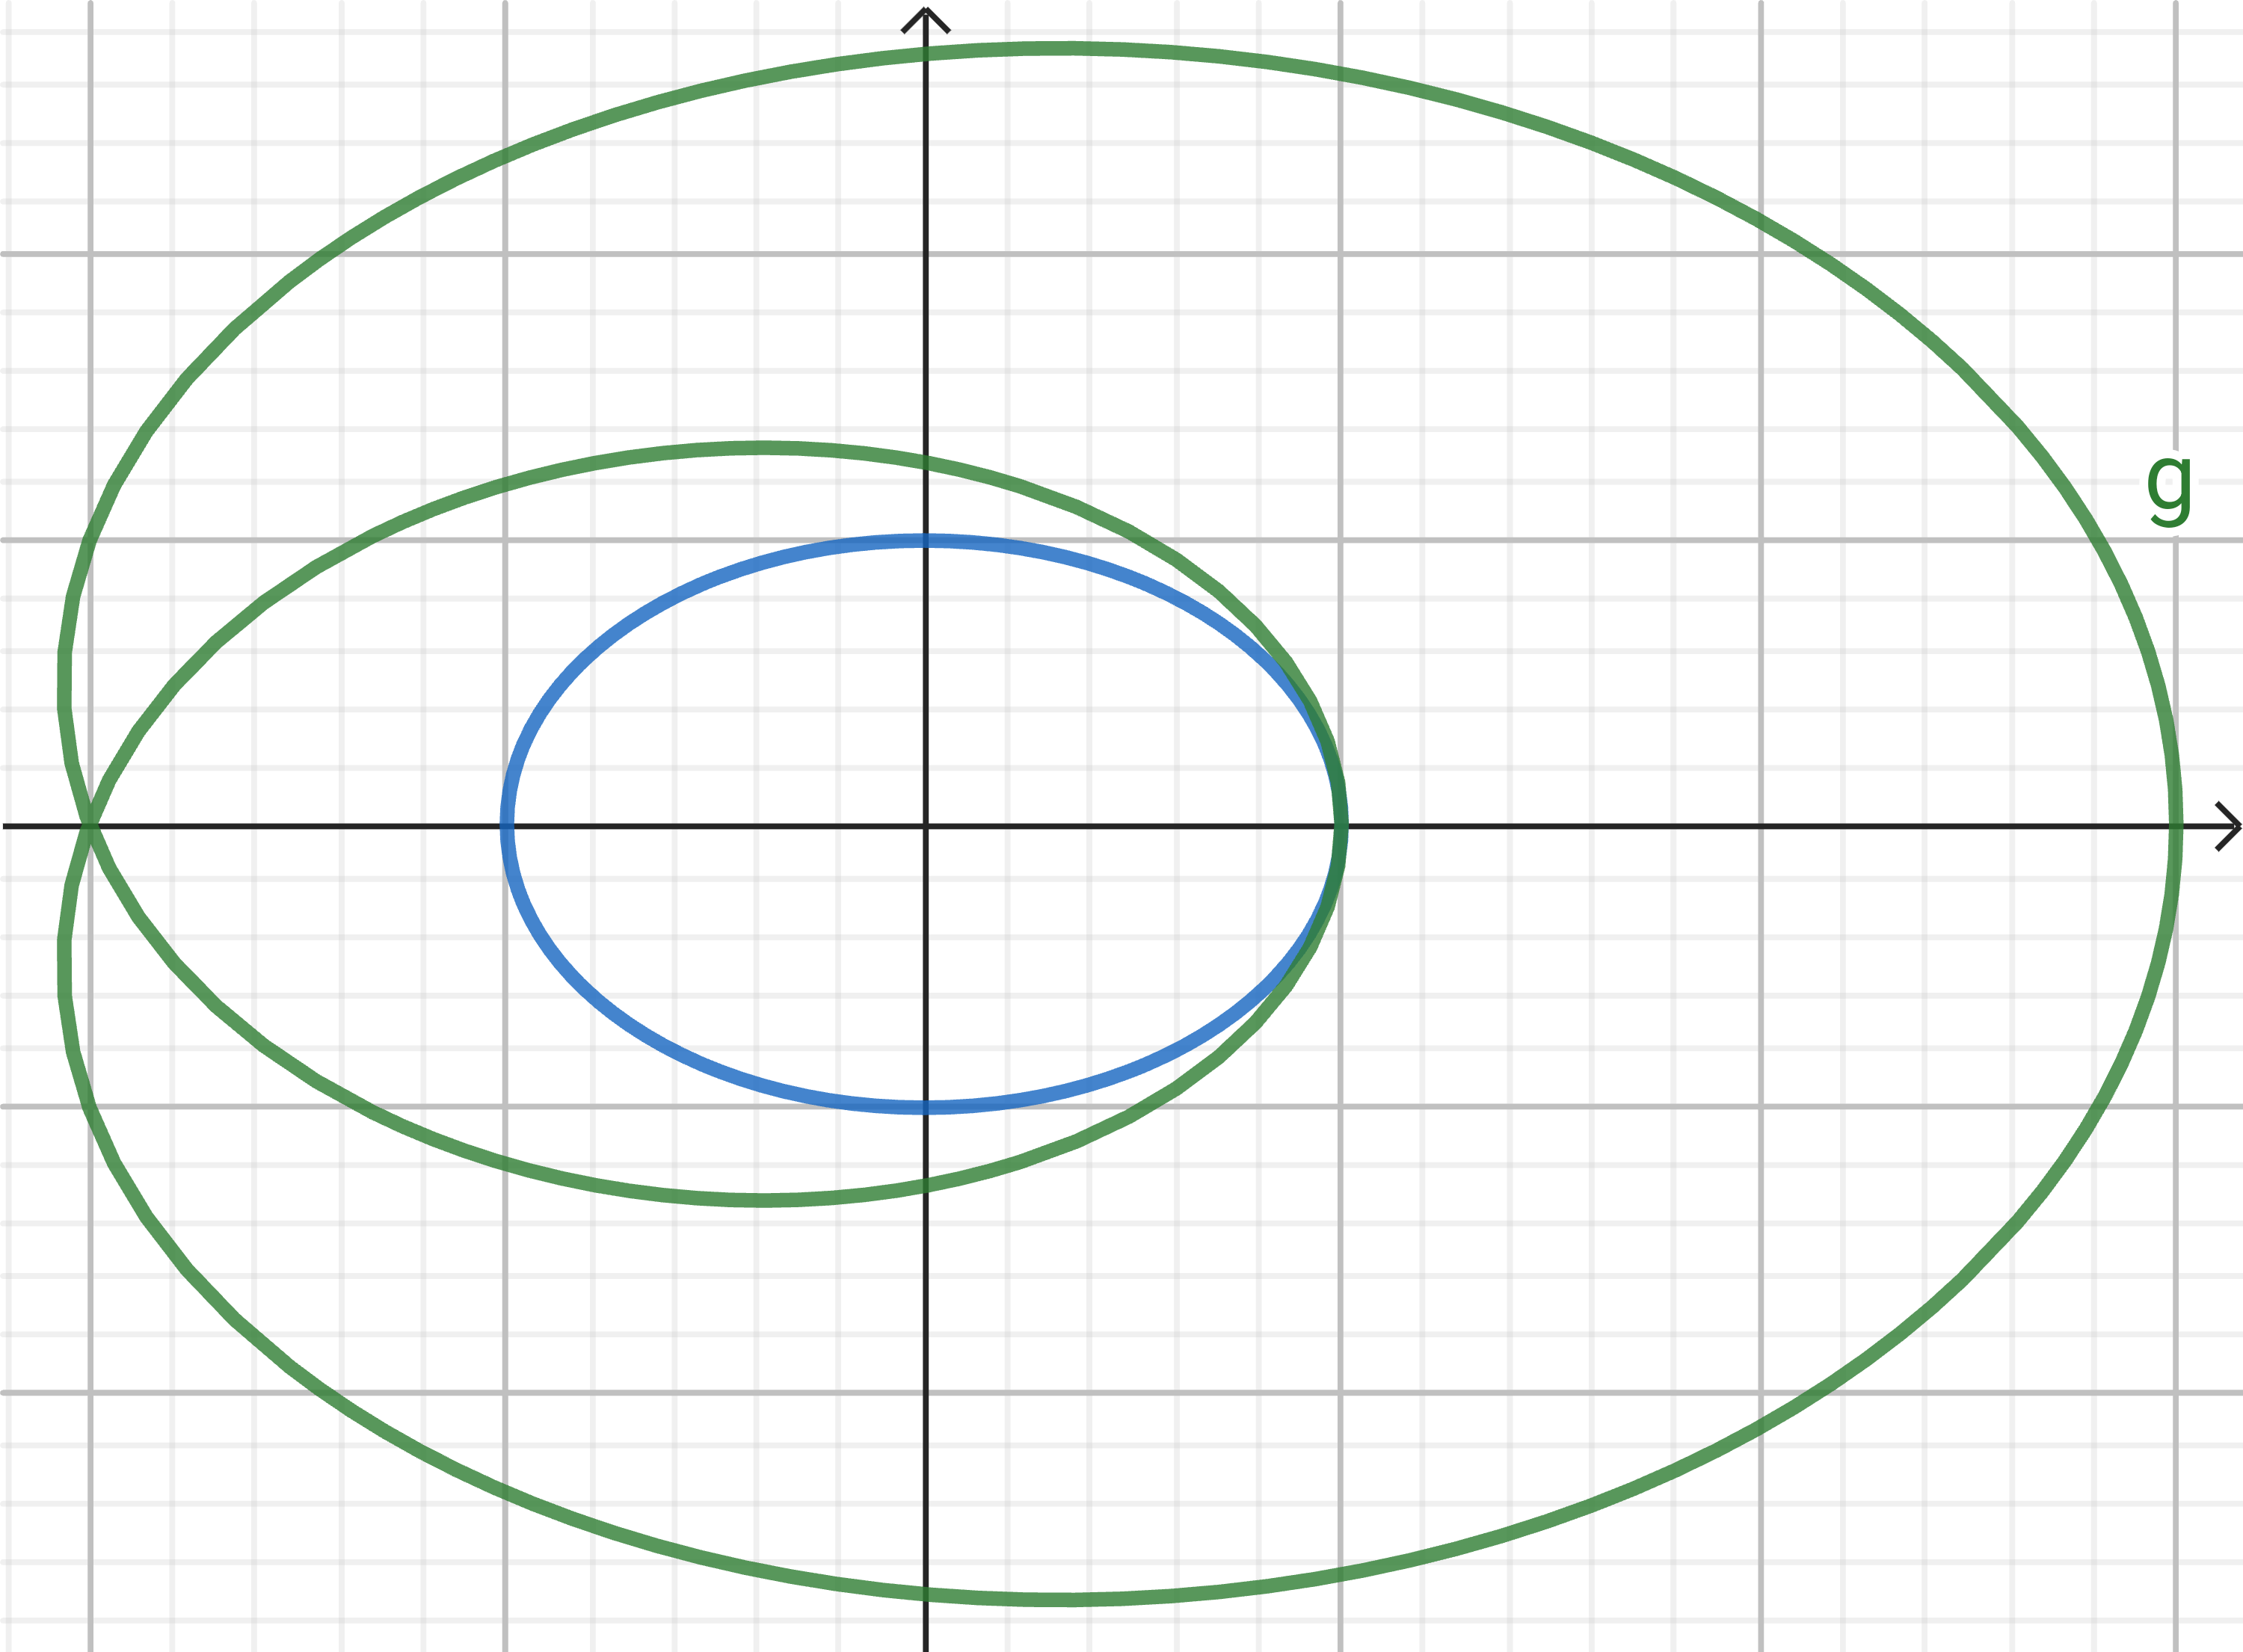
\includegraphics[width = 5cm]{homotopia.png}
\end{figure}

\begin{titlemize}{Lista de consequências}
	\item \hyperref[teo-fundamental-da-algebra]{teo-fundamental-da-algebra};\\ 
	
\end{titlemize}
